Galaxies, composed of stars, gas, and dust bound by gravitational forces, present complex patterns in their surface brightness distributions. Since its inception, the Hubble sequence \citep{hubble1982realm} has served as a cornerstone for classifying these celestial objects based on their morphological features, such as their elliptical shape, spiral arms or the presence of stellar central bars. However, the Hubble sequence has its limitations, including subjectivity in classification, a focus on superficial features rather than underlying physical properties, and a dependency on factors such as the galaxy's orientation (inclination) and the wavelength range of observations, rendering it incomplete for comprehensive astrophysical analysis.

Building on this foundation, photometric analysis of galaxy images has emerged as a robust tool for morphological analysis and classification, overcoming many limitations of the traditional classification.
%as each galaxy has a different superficial brightness distribution which depends in part on its morphology. 
As early as in the late 1980s, specialized software programs were developed to quantitatively analyze the brightness distribution of galaxies \citep{stetson1987daophot, mighell1989accurate}, allowing for a more objective and detailed understanding of their structure, which in turn shades light into their formation and evolution. Modern solutions like Imfit, developed by \citet{erwin2015imfit}, are contributing to the advancement of this field. Written in C++ and being open-source software, Imfit sets itself apart from older programs by going beyond radial profile analysis and being specifically designed for fitting 2D models into observational galaxy data images.
% It sets itself apart from older programs by going beyond radial profile analysis, incorporating Levenberg–Marquardt (L-M) gradient-search method for optimal fitting \citep{levenberg1944method, marquardt1963algorithm}. 



\begin{figure}
  \centering
  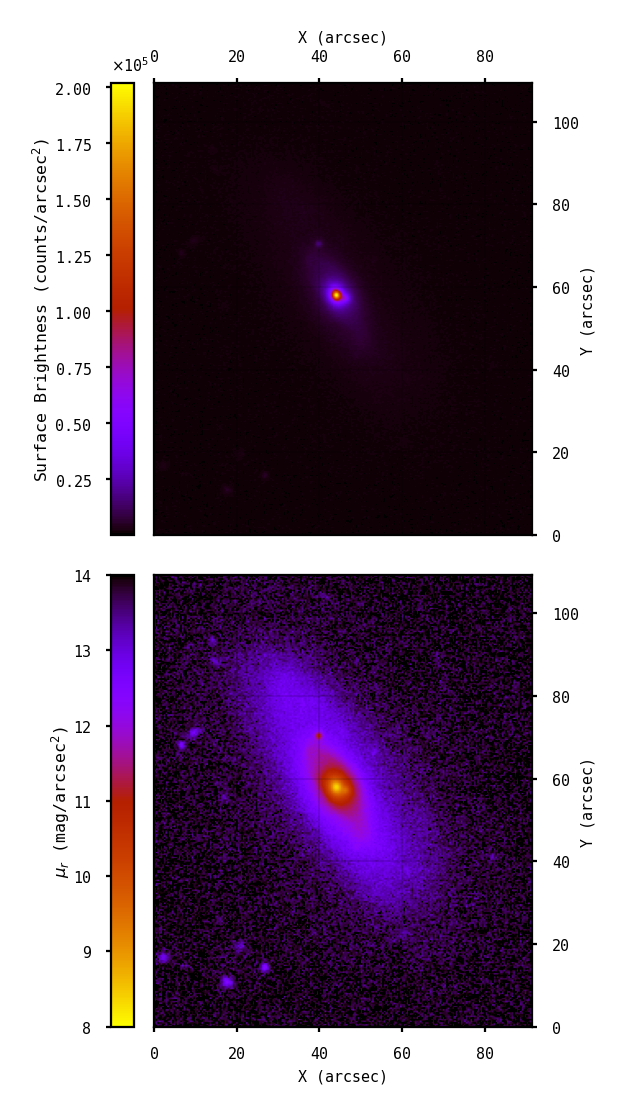
\includegraphics[width=1\columnwidth]{images/flux_mag_plot.png}  % adjust the width as you like
\caption{\small Near infrared ('i' band) image of UGC09629, observed on 2002-05-09 at Apache Point Observatory as a part of the Sloan Digital Sky Survey (SDSS). Exposure time was 53.91 seconds. (Top) surface brightness in counts per arcsecond$^2$. (Bottom) the same field in magnitudes per arcsecond squared. Axes of both figures are in arcseconds.}
  \label{fig:1}
\end{figure}

%

In the present study, we use Imfit to perform a photometric decomposition of the galaxy UGC09629 (see Figure \ref{fig:1}), situated in the constellation of Boötes, located in the northern celestial hemisphere as viewed from Earth at a declination of approximately 52 degrees north of the celestial equator. It is an Sa-type spiral galaxy with an estimated diameter of 60.31 kpc and it is receding from our Solar System at a velocity of approximately 7822 km s$^{-1}$ \citep{ned}. Based on the current (Planck satellite) value of the Hubble constant ($H_0=67.8 \ \text{km} \ \text{s}^{-1} \text{Mpc}^{-1}$) \citep{aghanim2020planck}, this translates to an estimated heliocentric distance of around $115.3$ Mpc. 

In the following sections, we construct and analyse three distinct 2D photometric models for the optimal fitting to discern UGC09629 morphological features. Isophotal profile analysis is also included. Finally, we discuss the limitations of our models and some potential improvements of our approach.




%¿Añadir expresión de Hubble?
%¿Imagen de la galaxia?
